%
% File acl2019.tex
%
%% Based on the style files for ACL 2018, NAACL 2018/19, which were
%% Based on the style files for ACL-2015, with some improvements
%%  taken from the NAACL-2016 style
%% Based on the style files for ACL-2014, which were, in turn,
%% based on ACL-2013, ACL-2012, ACL-2011, ACL-2010, ACL-IJCNLP-2009,
%% EACL-2009, IJCNLP-2008...
%% Based on the style files for EACL 2006 by 
%%e.agirre@ehu.es or Sergi.Balari@uab.es
%% and that of ACL 08 by Joakim Nivre and Noah Smith

\documentclass[11pt,a4paper]{article}
\usepackage[hyperref]{acl2019}
\usepackage{times}
\usepackage{latexsym}
\usepackage{graphicx} % include graphics
\usepackage{amsmath,amsfonts,amsthm,amssymb,amsopn,bm}
\usepackage{dsfont}
\usepackage{listings} % lstlisting
\usepackage{multirow}
\usepackage{tabularx}


\usepackage{url}

\aclfinalcopy % Uncomment this line for the final submission
%\def\aclpaperid{***} %  Enter the acl Paper ID here

%\setlength\titlebox{5cm}
% You can expand the titlebox if you need extra space
% to show all the authors. Please do not make the titlebox
% smaller than 5cm (the original size); we will check this
% in the camera-ready version and ask you to change it back.

\newcommand\BibTeX{B\textsc{ib}\TeX}
%%% math notations
\newcommand{\X}{\mathbf{X}}
\newcommand{\R}{\mathds{R}}

%%%%%%%%%%%%%%%%%%%%%%%%%%%%%%%%%%%%%%%%%%%%%%%%%%%%%%%%%%%
%% Lstlisting setting
%%%%%%%%%%%%%%%%%%%%%%%%%%%%%%%%%%%%%%%%%%%%%%%%%%%%%%%%%%%
\definecolor{codegreen}{rgb}{0,0.6,0}
\definecolor{codegray}{rgb}{0.5,0.5,0.5}
\definecolor{codepurple}{rgb}{0.58,0,0.82}
\definecolor{backcolour}{rgb}{0.95,0.95,0.92}
\lstdefinestyle{mystyle}{
    backgroundcolor=\color{backcolour},   
    commentstyle=\color{codegreen},
    keywordstyle=\color{magenta},
    numberstyle=\tiny\color{codegray},
    stringstyle=\color{codepurple},
    basicstyle=\footnotesize\sffamily,
    breakatwhitespace=false,         
    breaklines=true,                 
    captionpos=b,                    
    keepspaces=true,                 
    numbers=left,                    
    numbersep=5pt,                  
    showspaces=false,                
    showstringspaces=false,
    showtabs=false,                  
    tabsize=2 
}
\lstset{style=mystyle}


\title{Video Summarization}

\author{Ryan Rowe \\
  University of Washington \\ 
  \And
  Joseph Zhong \\
  University of Washington \\ 
  \texttt{\{rfrowe, josephz, prestonj\} @cs.washington.edu} \\
  \And
  Preston Jiang \\
  University of Washington \\ 
}

\date{}

\begin{document}
\maketitle
\begin{abstract}
    The use of recurrent neural networks with attention for processing time-sequential information, from audio, natural language processing, signal processing, as well as video processing has gained significant recent popularity, as this framework can be generalized to generate sequential outputs, such as captions. 
    In this paper, we propose a neural-based encoder-decoder method inspired with recent innovations incorporating attention mechanisms to re-weight the importance of encoded features across time. We deviate from this framework, instead, approaching discontinuities in input video contexts by directly detecting temporal boundaries in the encoding recurrent network.
    
    We provide our source code repository below\footnote{\url{https://github.com/joseph-zhong/VideoSummarization/}}.
\end{abstract}

\section{Introduction}


Every minute over 300 hours of video content are uploaded to YouTube.  This works out to nearly 50 years of new content each day.  The sheer amount of video data available–-thanks to the advent of the Internet-–on YouTube, Vimeo, Twitter, and hundreds of other websites means it is impossible for human eyes to watch each frame.  In order to quickly review massive amounts of video content, especially for long, multi-contextual videos such as surveillance videos, vlogs, or travel videos, one must first summarize each video.

In general, automatically describing video through human natural language is an important task in computer vision and machine learning: a similar and tangential task called video captioning extends towards a significant field of applications.

Many such video summarizers exist for various purposes.  For example, Descriptive Video Service (DVS) \cite{Dvs2019}  produces  video  descriptions  for  the  purpose  of  making  visual  media  such  as  television  or  films  more accessible to people of low-vision or other visual impairment \cite{Adp2019}. 

Analogous to video summarization, the tangentially related problem of captioning
has been applied to static images, or static visual captioning
\cite{DBLP:journals/corr/VinyalsTBE14, DBLP:journals/corr/KarpathyF14,
DBLP:journals/corr/XuBKCCSZB15, DBLP:journals/corr/VinyalsTBE16}. Such
techniques in image captioning have provided a fundamental basis for approaching
describing visual content in terms of natural language. As a result, this
approach has been extended to deal with the temporal progression of video
frames \cite{2015arXiv150208029Y, DBLP:journals/corr/SutskeverVL14,
DBLP:journals/corr/YuWHYX15}. 

Overall, past methods for video captioning and summarization have primarily
applied recurrent neural networks \cite{DBLP:journals/corr/abs-1808-03314,
DBLP:journals/corr/abs-1801-01078, DBLP:journals/corr/Lipton15} or long short-term memory neural
architectures \cite{hochreiter1997long, olah_2015}
which have been shown to be effective models for capturing the temporal
relationship between sequences of information. Naively applied, recurrent neural
networks and long short-term memory architectures can be effective for modelling
the sequential nature in time series data. However in the case of video
captioning, and in particular, complex edited videos with multiple segmented
points of short scenes, can have high variance in visual appearance, while still
maintaining contextual consistency \cite{DBLP:journals/corr/BaraldiGC16b}. 

Thus, in this paper we propose an architecture inspired by the work Baraldi et
al, \cite{DBLP:journals/corr/BaraldiGC16b} to use an attention-mechanism
inspired module to encode scene discontinuities in the video sequence. We report
experimentation on the Microsoft Video-to-Text (MSRVTT) dataset (see Figure \ref{fig:dataset})
\cite{inproceedings_Brad} containing over 200K video clip sentence-pairs. 

We organize our results as follows: we start our discussion with an overview of
previous methods in \S~2. In \S~3, we discuss our overall pipeline and
data representation. In \S~4, we discuss the details of our architecture
and the different neural models involved. In \S~5, we summarize our
experiment results, and finally in \S~6 we summarize weaknesses of our approach and future work in
video summarization.


%%% pipeline
\begin{figure*}
    \centering
    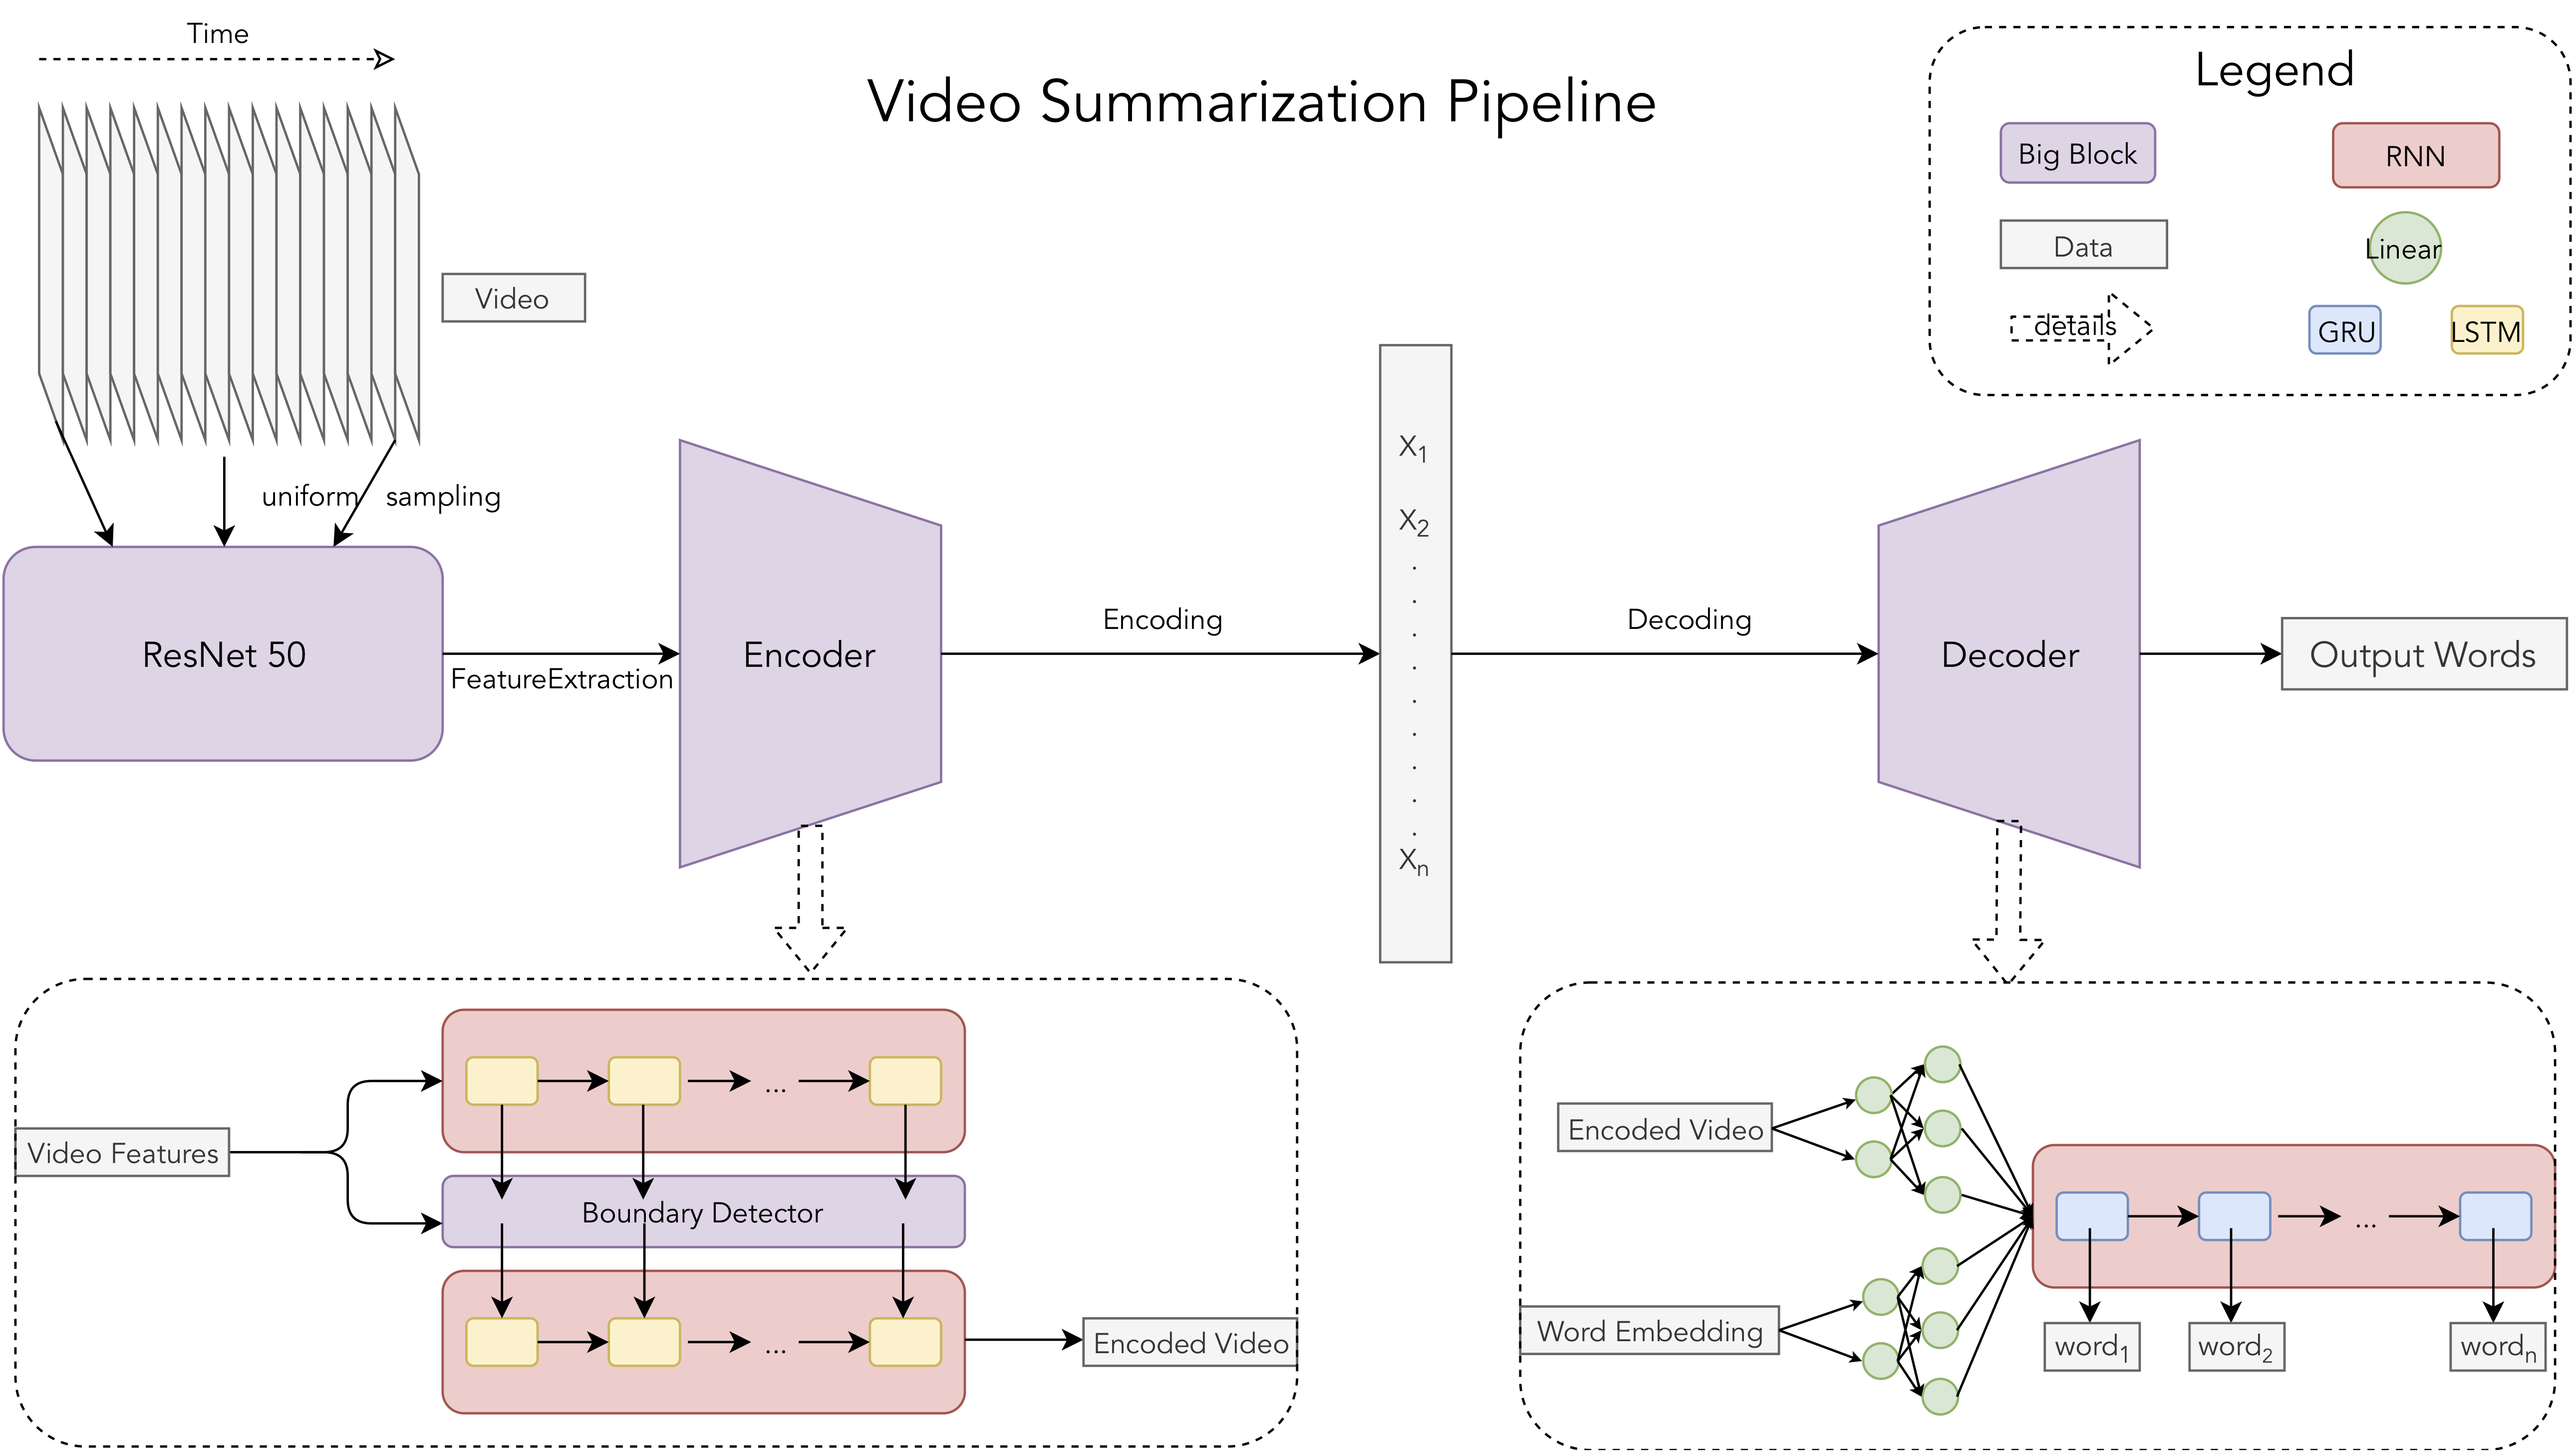
\includegraphics[scale=0.18]{pipeline.png}
    \caption{The video summarization pipeline. Video frames are uniformly sampled. ResNet50 \cite{DBLP:journals/corr/HeZRS15} is used to extract visual information of the frames. An Encoder-Decoder framework is used to generate text summaries from frames (see text for details).}
    \label{fig:pipeline}
\end{figure*}
%%%

\section{Related Works}

Early video captioning methods have entailed visual feature extraction to
condition the natural language captioning output in terms of subjects, objects,
and relational actions \cite{6c13e0e7819f435599f2cc315c48d790,
krishnamoorthy2013generating, C14-1115}. As an baseline approach, these methods
capture the basic, high-level content of an image, but cannot generalize to
complex sentences or unseen data outside the training dataset. Thus, this
motivates the application of more generalized decoders through recurrent neural
networks to better satisfy the rich natural language inherent in describing and
captioning complex video scenes \cite{DBLP:journals/corr/abs-1808-03314,
DBLP:journals/corr/abs-1801-01078, DBLP:journals/corr/Lipton15, hochreiter1997long, olah_2015}

One early approach in video captioning by
\citet{DBLP:journals/corr/VenugopalanXDRMS14}
motivated the use of recurrent neural networks to encode the sequence of
low-dimensional convolutional neural network features extracted from single
video frames, fed into a single LSTM layer. While effective in generally
encoding the visual content of the video frames, this method did not effectively
encode the sequential nature of the video input, framing video captioning data
into a static image captioning problem. Future work followed by encoding the
sequential transition using the \textit{sequence-to-sequence} approach in
recurrent neural architecture, encoding the sequential transitions in video
through a stacked LSTM architecture where subsequent layers of LSTM cells were
first conditioned by the outputs of the previous LSTM layers, inspired from work
in machine translation \cite{DBLP:journals/corr/SutskeverVL14}. 

As this general framework gained popularity, subsequent approaches incorporated
attention mechanisms in the sentence decoding \cite{2015arXiv150208029Y}, or
building visual-language semantic embeddings
\cite{DBLP:journals/corr/PanMYLR15}, or encoding external prior knowledge from
language models \cite{DBLP:journals/corr/VenugopalanHMS16}. 

More recently, research in video captioning has primarily focused on taking the
existing input representation and attempting to better exploit the internal
representation throughout the encoder-decoder neural architecture. \citet{DBLP:journals/corr/YuWHYX15} proposed a hierarchal recurrent neural architecture, where in
the sentence decoding, they introduced a sentence decoder as well as a paragraph
generator using a gated recurrent unit (GRU) layer
\cite{DBLP:journals/corr/ChoMGBSB14} while conditioning on contextual
information generated by the sentence generator, combined with the encoded video
features. 

In contrast, \citet{DBLP:journals/corr/PanXYWZ15} focused on video encoding, also using a
hierarchical approach to the recurrent video encoder. Similar to a
sliding-window approach, a LSTM is applied to over-lapping video chunks of
varying scales and granularities. 

In this paper, we take inspiration from  \citet{DBLP:journals/corr/BaraldiGC16b} to combine the
hierarchical architectures in both the encoder and decoder, while also
incorporating an attention-mechanism inspired boundary detection module in the
video encoder. The leveraging of
segment-level features has been previously investigated in natural language
processing \cite{DBLP:journals/corr/ChungAB16}, action recognition
\cite{tang_fei-fei_koller_2012, song_morency_davis_2013,
PirsiavashRamanan14CVPR, DBLP:journals/corr/LanZZS15} and
event detection context \cite{DBLP:journals/corr/WangXW0LTG16}. This technique
was first introduced to video captioning by \citet{DBLP:journals/corr/BaraldiGC16b}. We referenced
the implementations of the boundary detector from the \citet{banet2017} repository. 

\section{Approach}

%%% Figure Dataset sample
\begin{figure}
    \centering
    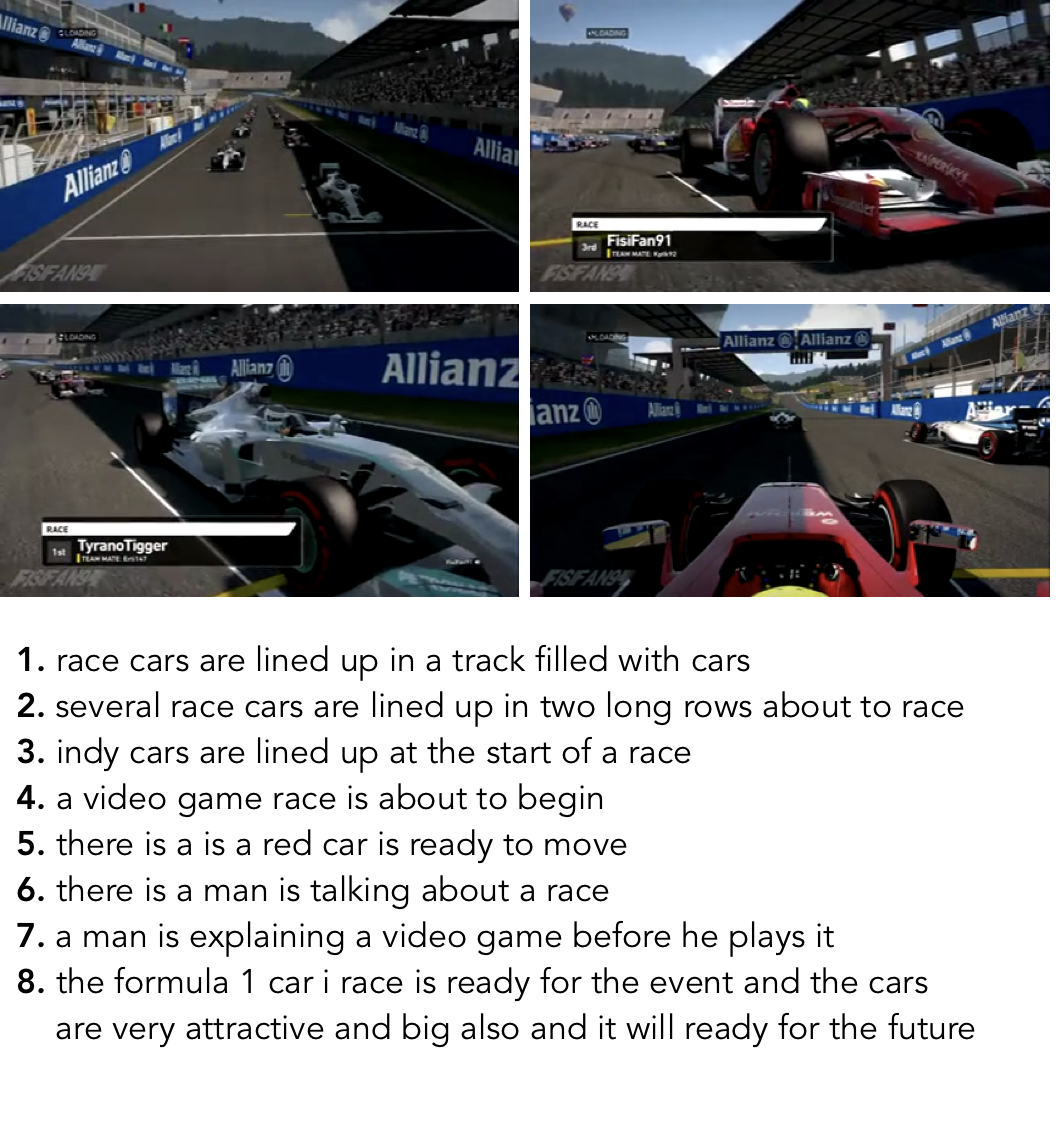
\includegraphics[width=\linewidth]{dataset.png}
    \caption{Example sample frames and label captions from the MSRVTT dataset \citet{Xu2016}}
    \label{fig:dataset}
\end{figure}

The overall architecture of our processing pipeline is described in Figure~\ref{fig:pipeline}. We uniformly sampled thirty frames for every video (to ensure this, we changed the sampling frequency with respect to each video's frame rate) to downsample the amount of repetitive frames in high refresh rate videos. First, for every video frame sampled, we used a pre-trained ResNet 50 \citet{DBLP:journals/corr/HeZRS15} network as the visual feature extractor and represented each video frame as the output of its last fully connected layer. Thus, we have out input $\X$ for each forward pass of our pipeline as 
\[\X \in \R^{N \times T \times p}\]
where $N$ is the batch size, $T$ is the sequence length (30), and $p$ is the dimensionality of the last fully connected layer of ResNet 50 (2048). 

Next, we used an Encoder-Decoder \cite{DBLP:journals/corr/ChoMGBSB14} architecture to transform video frame sequences to text summarization. For the encoder part, we used a two-layer recurrent neural network (RNN) with Long Short Term Memory (LSTM) cells \cite{hochreiter1997long}, sandwiching a boundary detector network, to encode the sequence information of the frames. The decoder consists of two fully connected networks to project the encoded frames and word embeddings and a RNN with Gated Recurrent Units (GRUs) \cite{DBLP:journals/corr/ChoMGBSB14}. The GRUs cells output the predicted words at such sequence step. 

The pipeline was trained tsinghrough cross entropy losses at each word prediction step, backpropagated from the decoder to the encoder. Note that we did \emph{not} adjust the weights of ResNet 50 using the cross entropy losses, as it only served as a feature extractor for the video frames. 

We discuss each part of this pipeline in detail in the next section. 

\section{Models}

\subsection{Encoder: LSTM + Boundary Detector}

For every input of the forward pass $X$, we first fed it into the first layer of the stacked LSTM. LSTM cells are defined through four ``gates'' which represent the short-term and long-term ``memory'' of how much information to forget and remember from the past. Specifically, the four gates are defined as:
\begin{align*}
    i_t &= \sigma(U^{(i)}x_t + W^{(i)}h_{t-1} + b^{(i)}) \\
    f_t &= \sigma(U^{(f)}x_t + W^{(f)}h_{t-1} + b^{(f)}) \\ 
    o_t &= \sigma(U^{(o)}x_t + W^{(o)}h_{t-1} + b^{(o)}) \\ 
    c_t &= f_t \circ c_{t-1} + i_t \circ \tilde{c_t}
\end{align*}
where $\tilde{c_t} = \text{tanh}(U^{(c)}x_t + W^{(c)}h_{t-1} + b^{(c)})$, and $h_t = o_t \circ \text{tanh}(c_t)$. Each $c_t$ is called a ``cell state'' and each $h_t$ is called a ``hidden state''. Assuming the hidden size of our LSTM network is $H$, we have our output from the first layer LSTM as $N\times T\times H$. 

We took the output of every hidden state cell of the first layer, and fed them into the Boundary Detector. The boundary detectors serves as a binary gate which decides if the hidden state from the LSTM should be result before being fed into the next one. The boundary detector is defined as 
\[s_t = \tau(\mathbf{v}^T_s \cdot [W_{si}x_t + W_{sh}h_{t-1} + b_s])\]
where 
\[\tau(x) =
\begin{cases}
1, &\text{if } \sigma(x) > 0.5 \\
0, &\text{otherwise}
\end{cases}\]
$\mathbf{v_s}, W_{si}, W_{sh}, b_s$ are learned parameters. In its essence, $s_t$ creates a binary mapping of the original hidden state and cell state to either keep or forget them. The input for the second layer LSTM, aka the hidden state and cell state from the previous layer, is in turn defined as 
\begin{align*}
h_{t-1} = h_{t-1} \cdot (1 - s_t) \\
c_{t-1} = c_{t-1} \cdot (1 - s_t)    
\end{align*}
We took the \emph{last} hidden output from the second layer LSTM as the encoding of the video frames. Therefore, our encoding has dimensionality $N \times H$. 

\subsection{Decoder: Fully connected layers + GRUs}
We first fed the encoded video frame, and word embedding into two fully connected layers respectively, which projects the dimentionality to $N \times P$, where $P$ is the output dimension. Then the output were added together to feed in the GRU cells. The GRU cells, similar to LSTM cells, are defined as 
\begin{align*}
    z_t &= \sigma(U^{(z)}x_t + W^{(z)}h_{t-1} + b^{(z)}) \\
    r_t &= \sigma(U^{(r)}x_t + W^{(r)}h_{t-1} + b^{(r)}) \\ 
    h_t &= (1 - z_t) \circ h_{t-1} + z_t \circ \tilde{h_t}
\end{align*}
where $\tilde{h_t} = \text{tanh}(U^{(h)}x_t + W^{(h)}(r_t \circ h_{t-1}) + b^{(h)})$. The actual words are then restored either through the $\arg\max$ of the hidden output at each step, or sampled using a multinomial distribution parameterized by the hidden output as the probabilities. Note that we used scheduled sampling \cite{Bengio:2015:SSS:2969239.2969370} during training period within a minimum ratio. 

For a complete summary of the dimension run-down through the pipeline, please refer to Table~\ref{tab:dim}.

\begin{table*}[t!]
\centering
\begin{tabular}{c|c|c}
\hline \textbf{Section} & \textbf{Component} & \textbf{Output Dimensionality} \\ \hline\hline
Feature Extraction & ResNet 50 & $N \times T \times p$ \\ \hline
\multirow{3}{*}{Encoding} & First Layer LSTM & $N \times T \times H$ \\
& Boundary Detector & $N \times T \times 1$ \\
& Second Layer LSTM & $N \times H$ \\ \hline
\multirow{3}{*}{Decoding} & Fully connected - Video Encoding & $ N \times P$ \\
& Fully connected - Word Embedding & $ N \times P$ \\
& GRU & $N \times \text{max words} $ \\
\hline
\end{tabular}
\caption{Each component in the processing pipeline and their output dimension. $N$: batch size; $T$: time steps (30 frames); $p$: the output dimension of ResNet 50; $H$: the hidden size of LSTM; $P$: the output dimension of the fully connected layers in the decoder; max words: the maximum length of the video caption prediction.}
\label{tab:dim}
\end{table*}

%%% result - med dataset
\begin{figure}
    \centering
    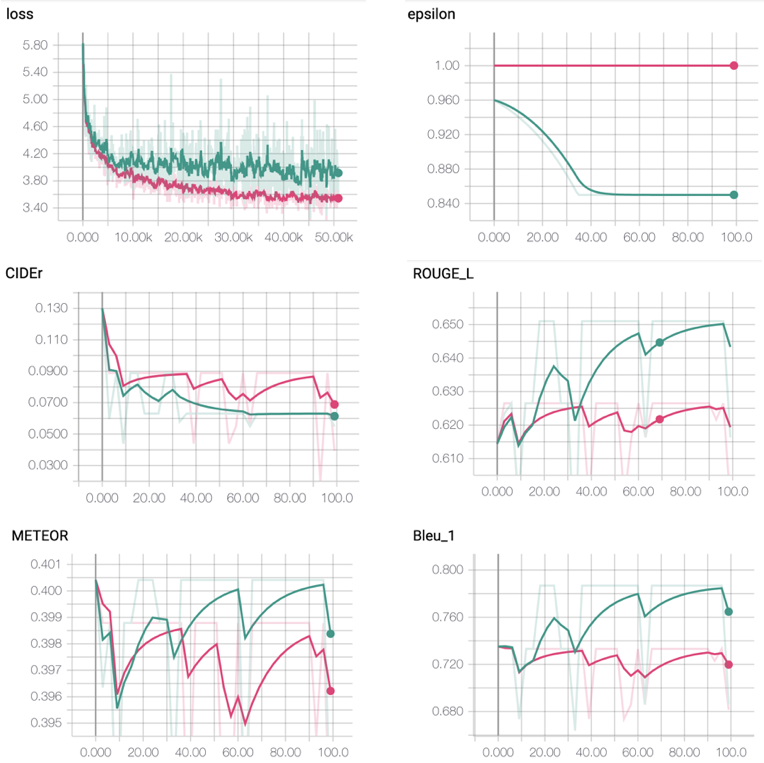
\includegraphics[width=\linewidth]{result_med.png}
    \caption{Results using a medium-size training set (25\% of MST-VTT), $\arg\max$ sampling for generating captions. Green curves have Teacher Forcing ratio 0.85, and red curves have Teaching Forcing ratio 1.0.}
    \label{fig:result_med}
\end{figure}
%%%

%%% result - large dataset
\begin{figure}
    \centering
    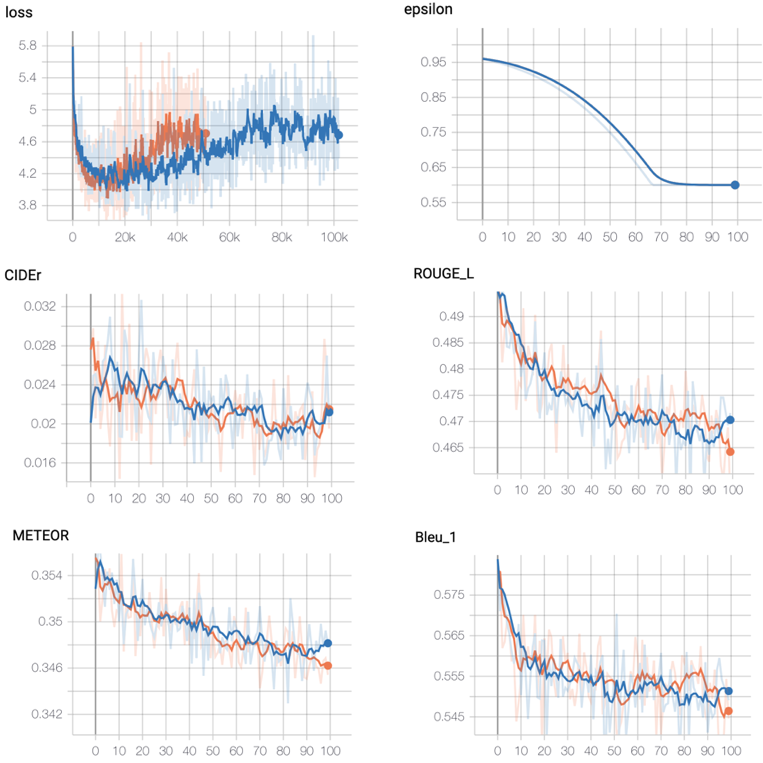
\includegraphics[width=\linewidth]{result_large.png}
    \caption{Results using multinomial sampling for generating words, and Teaching Forcing ratio of 0.6. Orange curves use a median-size dataset (25\% of MSR-VTT), blue curves use a large-size dataset (50\% of MSR-VTT).}
    \label{fig:result_large}
\end{figure}
%%%

%%% result - top k 
\begin{figure*}
    \centering
    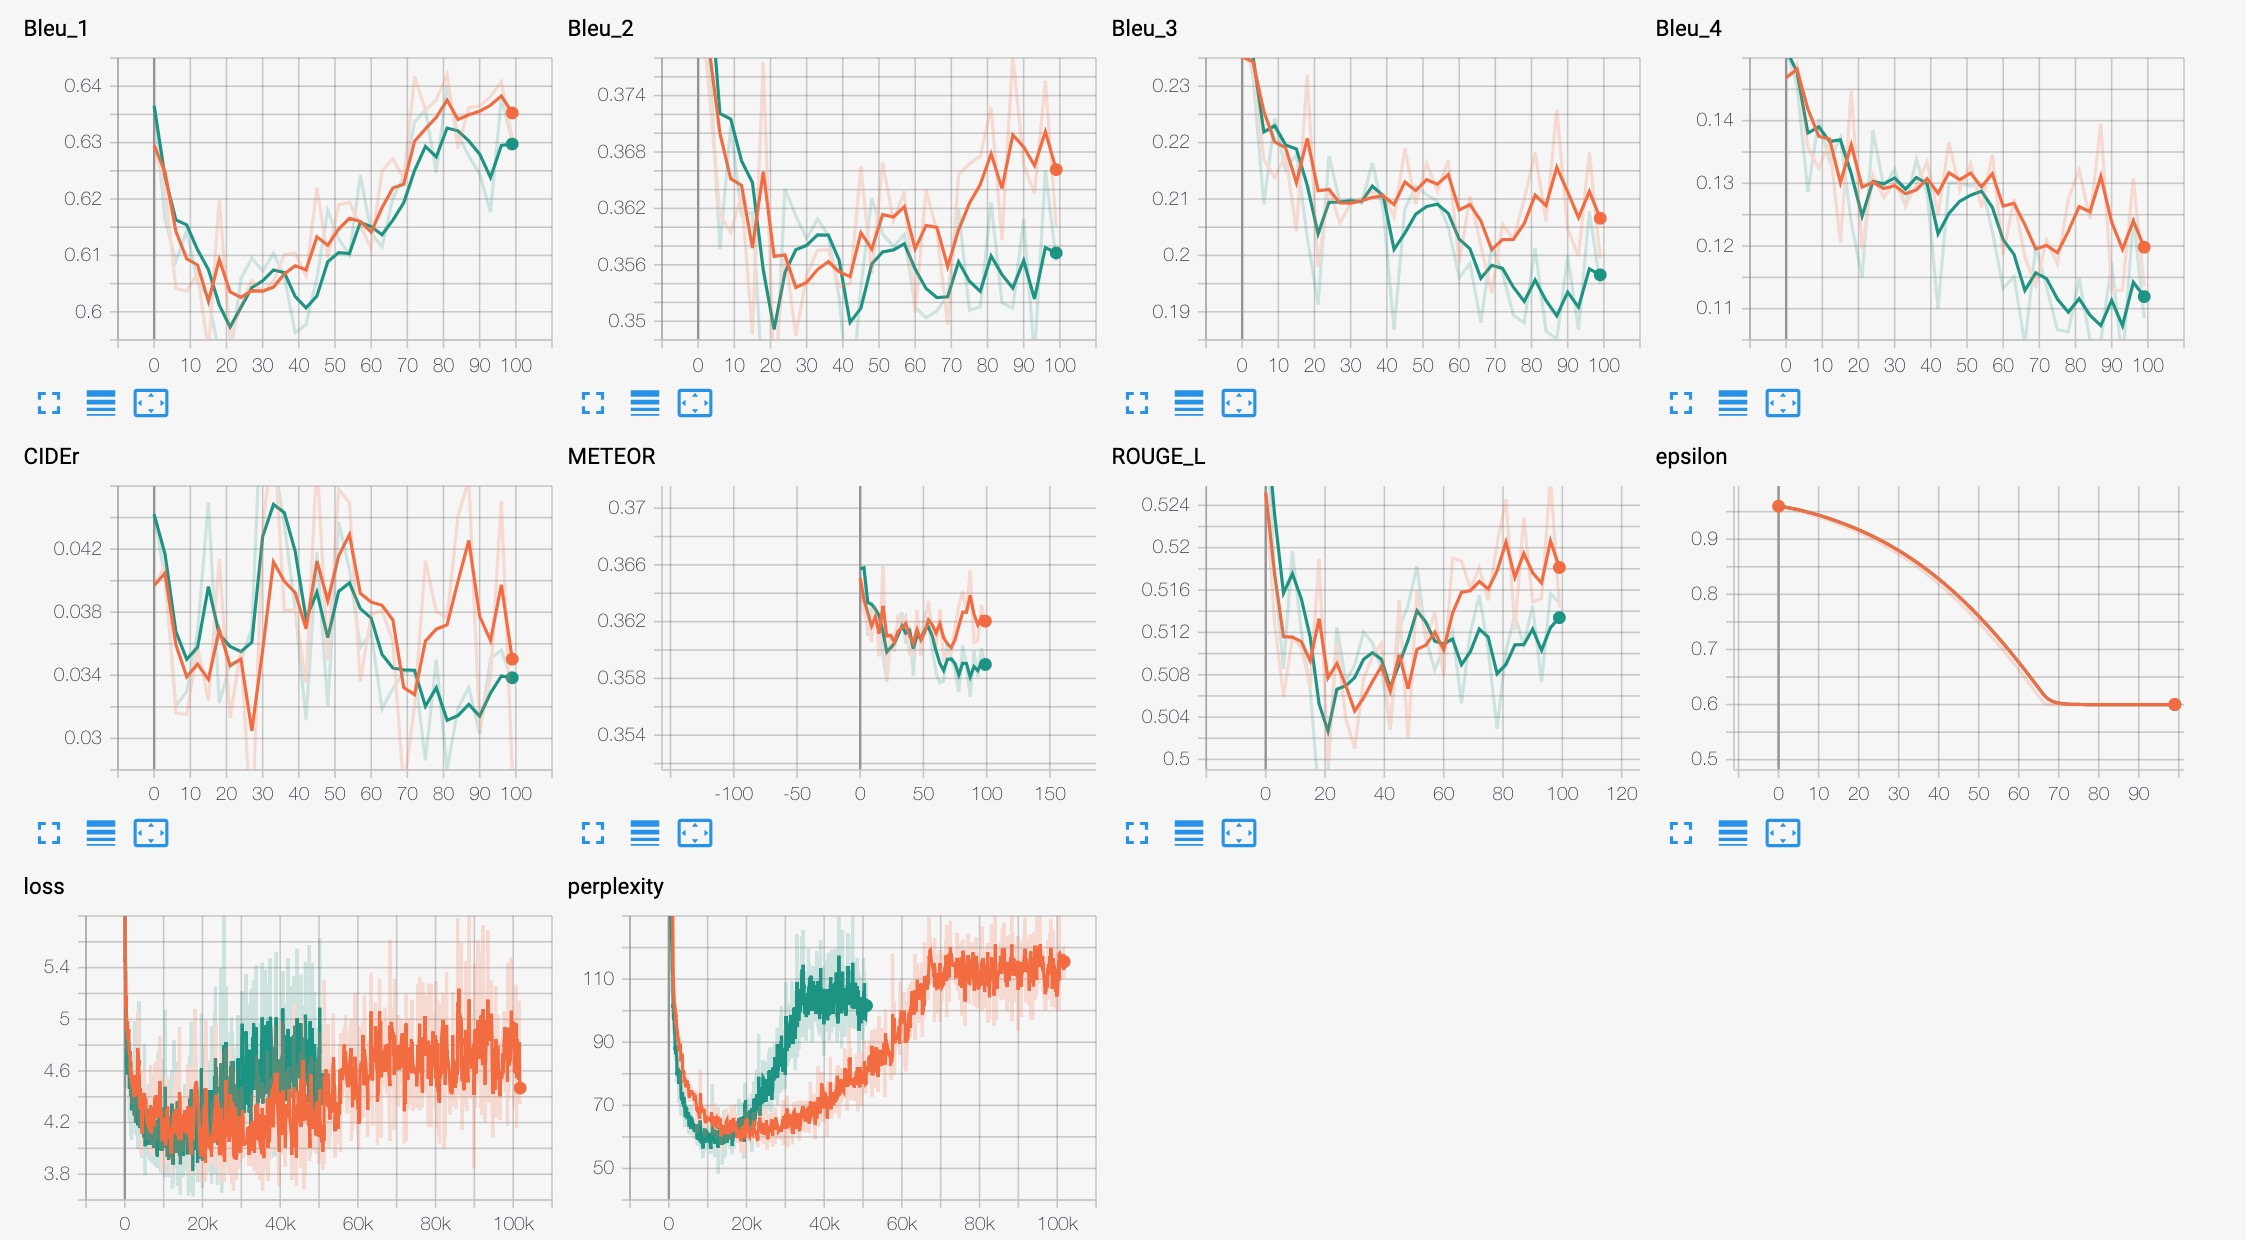
\includegraphics[width=\linewidth]{result_topk.jpg}
    \caption{Results using top-k ($k=20$ here) largest arguments as the multinomial probabilities for sampling to generate words, and Teaching Forcing ratio of 0.6. Green curves use a median-size dataset (25\% of MSR-VTT), oragne curves use a large-size dataset (50\% of MSR-VTT).}
    \label{fig:result_topk}
\end{figure*}
%%%

\section{Experiments and Results}

We report our results on the Microsoft Video-to-Text (MSRVTT) video-captioning dataset \citet{Xu2016}. 


%% Fuck yeah fuck Lamport.
%% Verbatim seems to make it go beyond the column?
\begin{figure}
\begin{lstlisting}
ground truth:
<start> a country music video <end>

top_k=20, min_ss=0.6:
<start> a woman is talking about the voice <end>

argmax, min_ss=0.85:
<start> a man is playing a song <end>

multinomial, min_ss=0.6:
<start> a scene of the wife s seeing <end>
\end{lstlisting}
\caption{Sample Output comparison between $\arg\max$, multinomial, and top-k multinomial sampling for \texttt{video7586} from the test set.}
\label{fig:output}
\end{figure}

In particular, we noticed that there were significant differences in the output based on the sampling strategy strategy, as well as the scheduled sampling teacher-forcing ratio. From Figure \ref{fig:result_med}, we report results on using our ``medium-size'' dataset, using about 25\% of the total MSR-VTT dataset, using $\arg\max$ sampling during caption decoding. Compared to Figures \ref{fig:result_large} and \ref{fig:result_topk}, the quantitative results in terms of evaluation metrics ``ROUGE\_L'', ``CIDEr'', ``METEOR'' and ``Bleu'' are significantly better and with seemingly better generalization, whereas the results from using ``multinomial'' or ``top-k multinomial'' sampling. However, this is counter intuitive, as multinomial sampling will produce much more diversified outputs. In fact, from our sample outputs in Figure \ref{fig:output}, we notice that the $\arg\max$ sampling strategy consistently outputs a ``averaged'' output, where a significant portion of the dataset actually consists of labels for where it is simply ``a man talking [...]'' (See Figure \ref{fig:dataset}). Thus, this actually informs us a significant issue with the MSR-VTT and its relationship with the evaluation metrics, where because a majority of the data samples contain such a general caption such as ``there is a man talking about a race'' (See Figure \ref{fig:dataset}). As a result, the ``multinomial'' and ``top-k'' results, while quantitatively seem significantly worse, produce more specific and nuanced results which deviate the label of ``a [wo]man talking about [...]''. See more results from Figure \ref{fig:output}.

\section{Conclusions and Future Work}

Overall, from the results we realize that there are two primary directions which simultaneously can significantly improve video summary generation. Firstly, we can tackle the neural architecture as motivated from previous works \citet{DBLP:journals/corr/BaraldiGC16b, 6c13e0e7819f435599f2cc315c48d790, DBLP:journals/corr/PanXYWZ15}, to better model the sequential nature of the video and exploit the context from the underlying temporal visual context, (e.g. attention mechanisms, automatic scene boundary detection). However, ultimately we suspect from our preprocessing pipeline of only using a pre-trained ImageNet \citet{imagenet_cvpr09} convolutional neural network (e.g. ResNet \citet{DBLP:journals/corr/HeZRS15}) to encode the features of the video fraem that there lies significant context to be extracted from significantly more semantically powerful and independent encoders. For example, we realized because the video sample from MSR-VTT have many captions which entirely deal in audio, that it would be a very fruitful future work to encode the audio context using both speech recognition encoders, as well as general audio scene classifiers, particularly with music videos with either singing or more culturally significant instrumental background music. 

Furthermore, beyond simply using pre-trained ImageNet encoders, we could also encode human action detection using 3D-convolutions \cite{Tran:2015:LSF:2919332.2919929}, using pretrained representations from video classification and spatio-temporal networks \citet{DBLP:journals/corr/abs-1711-10305, KarpathyCVPR14}. 

Lastly, recent works in language modeling have seen significant improvements through the evolution of attention mechanisms applied beyond recurrent neural architectures in the form of Transformer-based networks \citet{DBLP:journals/corr/abs-1810-04805, anonymous2019improving}, and could similarly enforce syntatically well-formed English captioning during decoding, rather than training the video caption decoder from scratch.

\section*{Acknowledgments}

We'd like to thank Professor Yejin Choi, and the assistants who helped and contributed greatly towards the quality of our education, Hannah Rashkin, Max Forbes, and Rowan Zellers.

\bibliography{acl2019}
\bibliographystyle{acl_natbib}




\end{document}
